%\documentclass[twocolumn, 10pt, aps, superscriptaddress, floatfix, showpacs, prl, citeautoscript]{revtex4-1}
\documentclass[10pt]{scrartcl}
%\documentclass[landscape,10pt]{scrartcl}



%%% PACKAGES %%%

% general
\usepackage[ngerman, english]{babel}
\usepackage[utf8]{inputenc}
%\usepackage[T1]{fontenc}
\usepackage{lmodern}
\usepackage{amssymb}
\usepackage{amsmath}
\usepackage{graphicx}

% page layout
\usepackage{geometry}                     % page layout, margins
%\usepackage[landscape]{geometry} % page layout, margins
%\geometry{a4paper, top=15mm, left=15mm, right=15mm, bottom=15mm, headsep=0mm, footskip=10mm}
\geometry{a4paper, top=20mm, bottom=20mm, left=20mm, right=20mm, footskip=10mm}
%\usepackage{fancyhdr} % header
%\pagestyle{fancy}           % header

% colors & hyperlinks
\usepackage[usenames,dvipsnames]{xcolor} % text colors
\usepackage[colorlinks, citecolor={blue!50!black}, urlcolor={blue!50!black}, linkcolor={red!50!black}]{hyperref}

% figures
%\usepackage{subfigure}   % subfigure
\usepackage{subcaption}  % subfigure
%\usepackage{floatflt}     % floating figure
\graphicspath{{figures/}} % Directory in which figures are stored

% tables
\usepackage{tabularx}                    % tables with manually set width
\usepackage{multirow, bigdelim}  % combine multiple rows in table, big delimiters
\usepackage{longtable}
%\usepackage{arydshln}                % dashed lines in table
\usepackage{makecell}                   % multi-line cells

% lists
\usepackage{mdwlist}      % list handling

% symbols etc.
\usepackage{verbatim}       % environment for interpreting all symbols as text, in tt font
\usepackage{bbm}              % double 1 for unit matrix \bbm{1}
%\usepackage[h]{esvect}   % vector arrows \vv{}
\usepackage{nicefrac}        % fractions with diagonal slash
%\usepackage{eurosym}    % Euro symbol €
\usepackage[vcentermath]{youngtab} % Young tableaux

% tools
\usepackage{etoolbox} % if-conditions in newcommand



%%% COMMANDS & MACROS %%%

% layout
%\setlength{\parindent}{0pt}       % no indent with new paragraph
\setcounter{tocdepth}{4}          % table of contents depth (to \paragraph)
\setcounter{secnumdepth}{4}  % depth of section numbers (to \paragraph 1.1.1.1.)

% table commands
\newcolumntype{L}[1]{>{\raggedright\arraybackslash}p{#1}} % linksbündig mit Breitenangabe
\newcolumntype{C}[1]{>{\centering\arraybackslash}p{#1}} % zentriert mit Breitenangabe
\newcolumntype{R}[1]{>{\raggedleft\arraybackslash}p{#1}} % rechtsbündig mit Breitenangabe

% colors
\definecolor{blau}{RGB}{0,84,159}
\definecolor{maigruen}{RGB}{189,205,0}
\definecolor{rot}{RGB}{204,7,30}
\definecolor{bordeaux}{RGB}{161,16,53}
\definecolor{violett}{RGB}{97,33,88}
\definecolor{lila}{RGB}{122,111,172}
\definecolor{magenta}{RGB}{255,0,255}
\definecolor{orange}{RGB}{255,140,0}

\definecolor{gelb}{RGB}{247,166,60}
\definecolor{gruen}{RGB}{85,170,67}
\definecolor{rot2}{RGB}{205,2,37}        %%%%
\definecolor{blau2}{RGB}{0,86,153}      %%%%

\newcommand{\bl}[1]{{\color{blau}{#1}}}
\newcommand{\vl}[1]{{\color{violett}{#1}}}
\newcommand{\gr}[1]{{\color{Green}{#1}}}
\newcommand{\rd}[1]{{\color{rot}{#1}}}
\newcommand{\bd}[1]{{\color{bordeaux}{#1}}}
\newcommand{\mg}[1]{{\color{magenta}{#1}}}
\newcommand{\ora}[1]{{\color{orange}{#1}}}


% Young tableaux macro
\newcommand{\y}[2]{
  \ifstrequal{#1}{0}
   {\ifstrequal{#2}{0}{$\bullet$}
    {\ifstrequal{#2}{1}{${\tiny \yng(1,1)}$}
     {\ifstrequal{#2}{2}{${\tiny \yng(2,2)}$}
      {${\tiny \yng(#1,#2)}$}
     }
    }
   }
   {\ifstrequal{#1}{1}
    {\ifstrequal{#2}{0}{${\tiny \yng(1)}$}
     {\ifstrequal{#2}{1}{${\tiny \yng(2,1)}$}
      {${\tiny \yng(#1,#2)}$}
     }
    }
    {\ifstrequal{#1}{2}
     {\ifstrequal{#2}{0}{${\tiny \yng(2)}$}
      {${\tiny \yng(#1,#2)}$}    
     }
    }
   }
}

% fraction macros
\newcommand{\f}[3]{$\frac{#1}{#2#3}$}
\newcommand{\fr}[2]{$\frac{#1}{#2}$}

% multi-line cells in table
\newcommand{\m}[1]{\multirow{2}{*}{#1}}
\newcommand{\mt}[1]{\multirow{3}{*}{#1}}
\newcommand{\mfour}[1]{\multirow{4}{*}{#1}}
\newcommand{\mfive}[1]{\multirow{5}{*}{#1}}
\newcommand{\msix}[1]{\multirow{6}{*}{#1}}
\newcommand{\mseven}[1]{\multirow{7}{*}{#1}}
\newcommand{\meight}[1]{\multirow{8}{*}{#1}}
\newcommand{\mten}[1]{\multirow{10}{*}{#1}}
\newcommand{\mtwelve}[1]{\multirow{12}{*}{#1}}

% big braces spanning several rows in table
\newcommand{\lb}{\ldelim\{{2}{*}}
\newcommand{\rb}{\rdelim\}{2}{*}}
\newcommand{\lbt}{\ldelim\{{3}{*}}
\newcommand{\lbfour}{\ldelim\{{4}{*}}
\newcommand{\lbfive}{\ldelim\{{5}{*}}
\newcommand{\lbsix}{\ldelim\{{6}{*}}
\newcommand{\lbseven}{\ldelim\{{7}{*}}
\newcommand{\lbeight}{\ldelim\{{8}{*}}


% macros for Green's functions and vertex functions
\newcommand{\G}[6]{
	\ifstrequal{#6}{0101}
		{#1^{\alpha_#2 | \alpha_#3^\prime}_{\sigma_#4 | \sigma_#5^\prime}}
	{\ifstrequal{#6}{0100}
		{\ifstrequal{#4}{#5}
			{#1^{\alpha_#2 | \alpha_#3^\prime}_{\sigma_#4}}
			{#1^{\alpha_#2 | \alpha_#3^\prime}_{\sigma_#4 | \sigma_#5}}
		}
	{\ifstrequal{#6}{1000}
		{\ifstrequal{#4}{#5}
			{#1^{\alpha_#2^\prime | \alpha_#3}_{\sigma_#4}}
			{#1^{\alpha_#2^\prime | \alpha_#3}_{\sigma_#4 | \sigma_#5}}
		}
	{0}
	}}
}

\newcommand{\gqw}[5]{
	\ifstrequal{#5}{1010}
		{\!\left(
		 q_#1^\prime | q_#2 \,,\,
		 \omega_#3^\prime | \omega_#4
		 \right)}
	{\ifstrequal{#5}{0101}
		{\!\left(
		 q_#1 | q_#2^\prime \,,\,
		 \omega_#3 | \omega_#4^\prime
		 \right)}
	{\ifstrequal{#5}{1000}
		{\ifstrequal{#3}{#4}
			{\!\left(
			 q_#1^\prime | q_#2 \,,\,
			 \omega_#3
			 \right)}
			 {\!\left(
			 q_#1^\prime | q_#2 \,,\,
			 \omega_#3 | \omega_#4
			 \right)}
		}
	{\ifstrequal{#5}{0100}
		{\ifstrequal{#3}{#4}
			{\!\left(
			 q_#1 | q_#2^\prime \,,\,
			 \omega_#3
			 \right)}
			 {\!\left(
			 q_#1 | q_#2^\prime \,,\,
			 \omega_#3 | \omega_#4
			 \right)}
		}
	{0}
	}}}
}

\newcommand{\V}[9]{
	\def\Vertex{#1}
	\def\ala{#2}
	\def\alb{#3}
	\def\alc{#4}
	\def\ald{#5}
	\def\sga{#6}
	\def\sgb{#7}
	\def\sgc{#8}
	\def\sgd{#9}
	\Vcont
}
% indices have: 
% 0 = nothing
% 1 = prime
% 2 = bar
% 3 = prime + bar
% 4 = (no bar, bar)
% 5 = prime + (no bar, bar)
% 6 = (bar, no bar)
% 7 = prime + (bar, no bar)
\newcommand{\Vcont}[1]{
	\ifstrequal{#1}{1010}
		{\Vertex
		 ^{\alpha_\ala^\prime \alpha_\alb^\prime | \alpha_\alc \alpha_\ald}
		 _{\sigma_\sga^\prime \sigma_\sgb^\prime | \sigma_\sgc \sigma_\sgd}\,}
	{\ifstrequal{#1}{1000}
		{\Vertex
		 ^{\alpha_\ala^\prime \alpha_\alb^\prime | \alpha_\alc \alpha_\ald}
		 _{\sigma_\sga \sigma_\sgb | \sigma_\sgc \sigma_\sgd}\,}
	{\ifstrequal{#1}{0100}
		{\Vertex
		 ^{\alpha_\ala \alpha_\alb | \alpha_\alc^\prime \alpha_\ald^\prime}
		 _{\sigma_\sga \sigma_\sgb | \sigma_\sgc \sigma_\sgd}\,}
	{\ifstrequal{#1}{0101}
		{\Vertex
		 ^{\alpha_\ala \alpha_\alb | \alpha_\alc^\prime \alpha_\ald^\prime}
		 _{\sigma_\sga \sigma_\sgb | \sigma_\sgc^\prime \sigma_\sgd^\prime}\,}
	{\ifstrequal{#1}{1011}
		{\Vertex
		 ^{\alpha_\ala^\prime \alpha_\alb^\prime | \alpha_\alc \alpha_\ald}
		 _{\sigma_\sga^\prime \sigma_\sgb^\prime | \sigma_\sgc^\prime \sigma_\sgd^\prime}\,}
	{\ifstrequal{#1}{1032}
		{\Vertex
		 ^{\alpha_\ala^\prime \alpha_\alb^\prime | \alpha_\alc \alpha_\ald}
		 _{\bar{\sigma}_\sga^\prime \bar{\sigma}_\sgb^\prime | \bar{\sigma}_\sgc \bar{\sigma}_\sgd}\,}
	{\ifstrequal{#1}{1033}
		{\Vertex
		 ^{\alpha_\ala^\prime \alpha_\alb^\prime | \alpha_\alc \alpha_\ald}
		 _{\bar{\sigma}_\sga^\prime \bar{\sigma}_\sgb^\prime | \bar{\sigma}_\sgc^\prime \bar{\sigma}_\sgd^\prime}\,}
	{\ifstrequal{#1}{1054}
		{\Vertex
		 ^{\alpha_\ala^\prime \alpha_\alb^\prime | \alpha_\alc \alpha_\ald}
		 _{\sigma_\sga^\prime \bar{\sigma}_\sgb^\prime | \sigma_\sgc \bar{\sigma}_\sgd}\,}
	{\ifstrequal{#1}{1044}
		{\Vertex
		 ^{\alpha_\ala^\prime \alpha_\alb^\prime | \alpha_\alc \alpha_\ald}
		 _{\sigma_\sga \bar{\sigma}_\sgb | \sigma_\sgc \bar{\sigma}_\sgd}\,}
	{\ifstrequal{#1}{1055}
		{\Vertex
		 ^{\alpha_\ala^\prime \alpha_\alb^\prime | \alpha_\alc \alpha_\ald}
		 _{\sigma_\sga^\prime \bar{\sigma}_\sgb^\prime | \sigma_\sgc^\prime \bar{\sigma}_\sgd^\prime}\,}
	{\ifstrequal{#1}{1066}
		{\Vertex
		 ^{\alpha_\ala^\prime \alpha_\alb^\prime | \alpha_\alc \alpha_\ald}
		 _{\bar{\sigma}_\sga \sigma_\sgb | \bar{\sigma}_\sgc \sigma_\sgd}\,}
	{\ifstrequal{#1}{1077}
		{\Vertex
		 ^{\alpha_\ala^\prime \alpha_\alb^\prime | \alpha_\alc \alpha_\ald}
		 _{\bar{\sigma}_\sga^\prime \sigma_\sgb^\prime | \bar{\sigma}_\sgc^\prime \sigma_\sgd^\prime}\,}
	{\ifstrequal{#1}{10cc}
		{\Vertex
		 ^{\alpha_\ala^\prime \alpha_\alb^\prime | \alpha_\alc \alpha_\ald}
		 _{\sigma \sigma | \sigma \sigma}\,}
	{\ifstrequal{#1}{10dd}
		{\Vertex
		 ^{\alpha_\ala^\prime \alpha_\alb^\prime | \alpha_\alc \alpha_\ald}
		 _{\sigma \bar{\sigma} | \sigma \bar{\sigma}}\,}
	{\ifstrequal{#1}{10ee}
		{\Vertex
		 ^{\alpha_\ala^\prime \alpha_\alb^\prime | \alpha_\alc \alpha_\ald}
		 _{\sigma \bar{\sigma} | \bar{\sigma} \sigma}\,}
	{0}
	}}}}}}}}}}}}}}
}

\newcommand{\vqw}[8]{
	\def\qa{#1}
	\def\qb{#2}
	\def\qc{#3}
	\def\qd{#4}
	\def\wa{#5}
	\def\wb{#6}
	\def\wc{#7}
	\def\wd{#8}
	\vqwcont
}
\newcommand{\vqwcont}[1]{
	\ifstrequal{#1}{1010}
		{\!\left(
		 q_\qa^\prime q_\qb^\prime | q_\qc q_\qd \,,\,
		 \omega_\wa^\prime \omega_\wb^\prime | \omega_\wc \omega_\wd
		 \right)}
	{\ifstrequal{#1}{0101}
		{\!\left(
		 q_\qa q_\qb| q_\qc^\prime  q_\qd^\prime \,,\,
		 \omega_\wa \omega_\wb | \omega_\wc^\prime  \omega_\wd^\prime 
		 \right)}
	{\ifstrequal{#1}{1000}
		{\!\left(
		 q_\qa^\prime q_\qb^\prime | q_\qc q_\qd \,,\,
		 \omega_\wa \omega_\wb | \omega_\wc \omega_\wd
		 \right)}
	{\ifstrequal{#1}{0100}
		{\!\left(
		 q_\qa q_\qb| q_\qc^\prime  q_\qd^\prime \,,\,
		 \omega_\wa \omega_\wb | \omega_\wc  \omega_\wd
		 \right)}
	{0}
	}}}
}


\newcommand{\Ktot}[1]{\mathcal{K}_#1}
\newcommand{\K}[2]{\mathcal{K}_#1^#2}
\newcommand{\Kb}[2]{\mathcal{K}_{#1^\prime}^{#2}}


% frequency integral macro
\newcommand{\intw}[1]{\int \! \mathrm{d} \omega_#1}

% large sums macro
\newcommand{\lsum}[3]{\sum_{\substack{#1_#2 #1_#3 \\ #1_#2^\prime #1_#3^\prime}}\ }
\newcommand{\lsumt}[3]{\sum_{#1_#2 #1_#3}\ }

% Dirac delta, Kronecker delta
\newcommand{\delomegap}[2]{\delta(\omega_#1 - \omega_#2^\prime)\,}
\newcommand{\delsigma}[2]{\delta_{\sigma_#1 \sigma_#2}\,}
\newcommand{\delsigmap}[2]{\delta_{\sigma_#1^\prime \sigma_#2}\,}
\newcommand{\delsigmapp}[2]{\delta_{\sigma_#1^\prime \sigma_#2^\prime}\,}


\newcommand{\updown}{_{\uparrow\downarrow}}

%%% DOCUMENT %%%

\begin{document}

\section*{Zero-frequency perturbation theory}

We show all diagrams of the vertex $\Gamma\updown$ in perturbation theory up to $4^\text{th}$ order, and the values of their fully retarded components (only one Keldysh index is 1) at all frequencies equal to zero, $\Gamma\updown(0,0,0,0)$, computed with the Keldysh-mfRG code. The fully advanced components (only one Keldysh index is 2) have the same value (since it is real) at the particle-hole symmetric point. Analytical results, where available, are due to Hewson, J. Phys.: Condens. Matter \textbf{13}, 10011 (2001).

Different colors indicate the spin: Dark blue corresponds to $\uparrow$, light blue to $\downarrow$. The spin of green lines is summed over (separately for each green $p$ bubble), with dark and light green lines having opposite spins.

We do not display prefactors: Every $t$ bubble implies a minus sign, and all $p$ bubbles have a prefactor of $1/2$.

\subsection*{1$^\text{st}$ and 2$^\text{nd}$ order}

\begin{figure}[h!]
\begin{subfigure}[c]{0.4\textwidth}
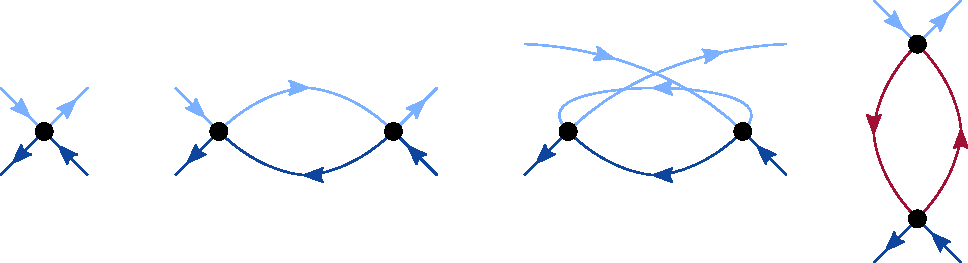
\includegraphics[scale=0.3]{diagrams/PT2}
\\
$\Gamma_0$ \hspace{0.75cm} $\K1a$ \hspace{1.1cm} $\K1p$ \hspace{0.7cm} $\K1t$
\end{subfigure}
\begin{subfigure}[c]{0.4\textwidth}
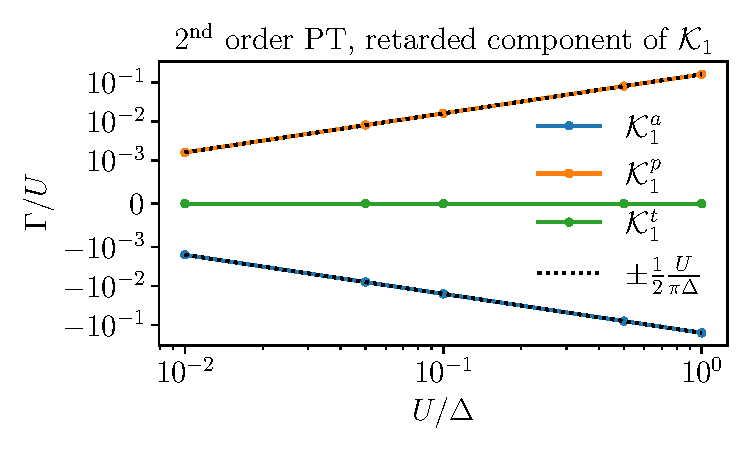
\includegraphics[scale=0.65]{plots/PT2}
\end{subfigure}
\caption{Vertex diagrams in $1^\text{st}$ (bare vertex $\Gamma_0$) and $2^\text{nd}$ order (only $\Ktot1$ diagrams). ${\K1t}\updown$ is zero, since the red lines can have neither spin $\uparrow$ nor $\downarrow$. Diagrams in the $a$ and $p$ channel cancel.}
\end{figure}

\newpage

\subsection*{3$^\text{rd}$ order}

\vspace{-0.5cm}

\begin{figure}[h!]
\begin{subfigure}[c]{0.4\textwidth}
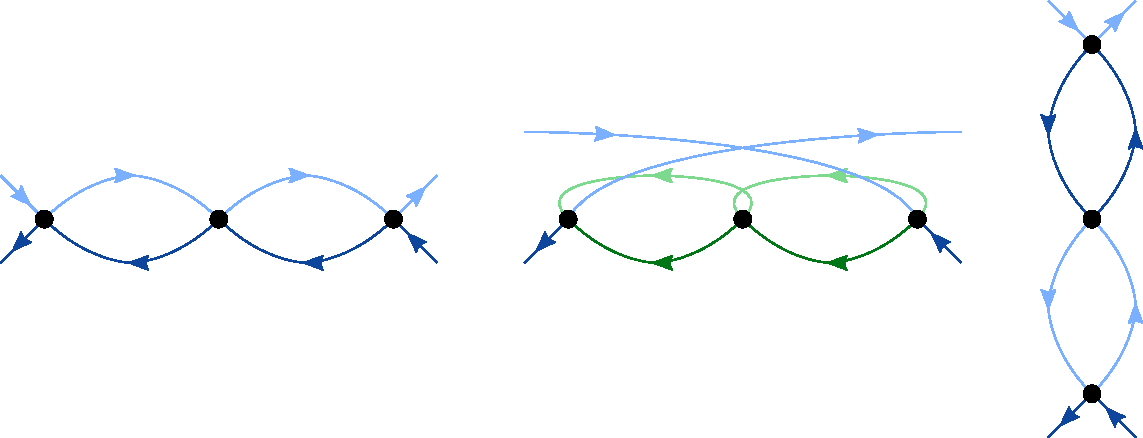
\includegraphics[scale=0.3]{diagrams/PT3_K1}
\\
\phantom{.}\hspace{0.75cm} $\K1a$ \hspace{2cm} $\K1p$ \hspace{1cm} $\K1t$
\end{subfigure}
\begin{subfigure}[c]{0.4\textwidth}
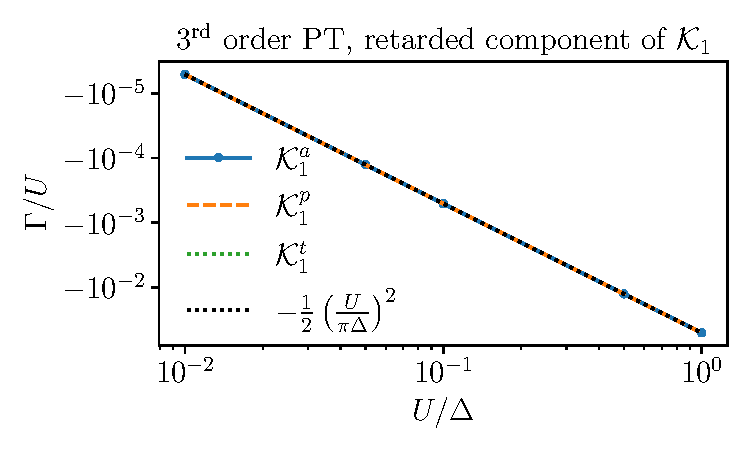
\includegraphics[scale=0.65]{plots/PT3_K1}
\end{subfigure}
\caption{$\Ktot1$ diagrams in $3^\text{rd}$ order. All three diagrams give the same result.}
\end{figure}

\vspace{-0.5cm}

\begin{figure}[h!]
\begin{subfigure}[c]{0.4\textwidth}
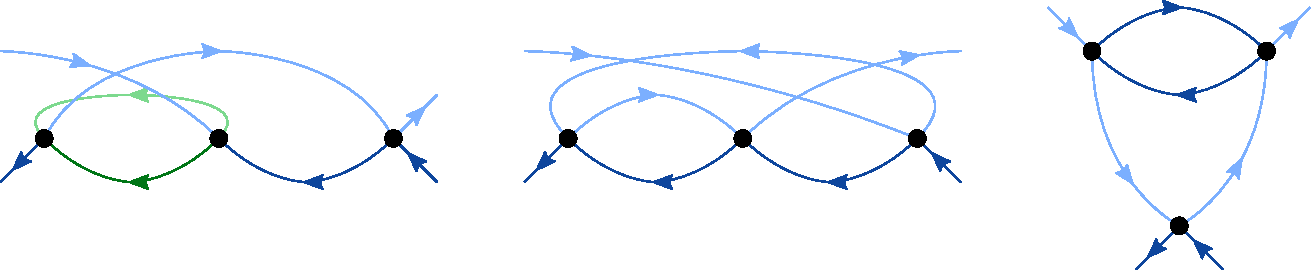
\includegraphics[scale=0.3]{diagrams/PT3_K2}
\\
\phantom{.}\hspace{0.75cm} $\K2a$ \hspace{2cm} $\K2p$ \hspace{1.5cm} $\K2t$
\\ \\
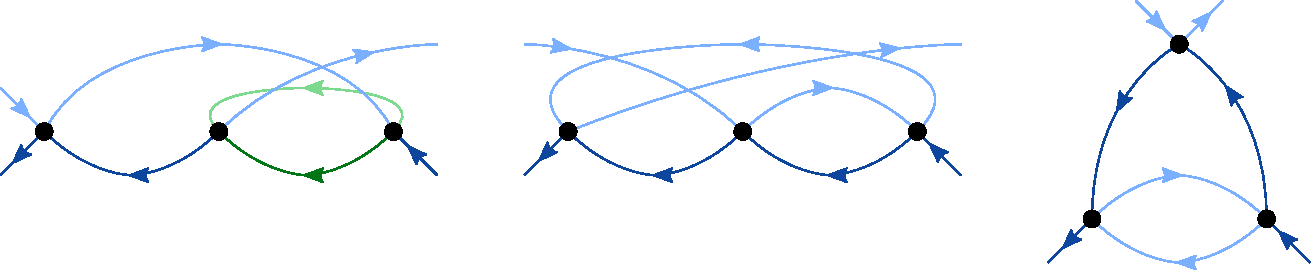
\includegraphics[scale=0.3]{diagrams/PT3_K2b}
\\
\phantom{.}\hspace{0.75cm} $\Kb2a$ \hspace{1.9cm} $\Kb2p$ \hspace{1.4cm} $\Kb2t$
\end{subfigure}
\begin{subfigure}[c]{0.4\textwidth}
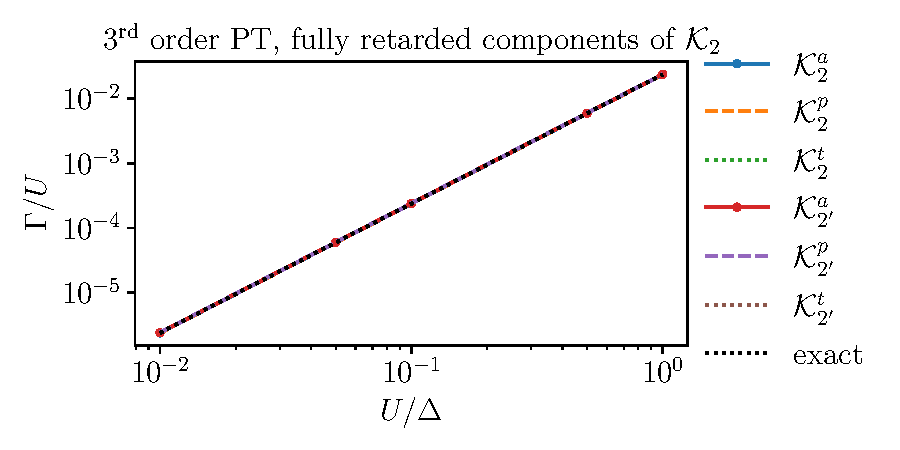
\includegraphics[scale=0.65]{plots/PT3_K2}
\end{subfigure}
\caption{$\Ktot2$ (top row) and $\Ktot{{2^\prime}}$ (bottom row) diagrams in $3^\text{rd}$ order. For diagrams not appearing here, the $\uparrow\downarrow$ component is zero due to the spin structure (cf.~$\K1t$ in $2^\text{nd}$ order). All diagrams give the same result, the exact analytical value is $\K{{2^{(\prime)}}}{r}=-\frac{1}{2}(2\!-\!\frac{\pi^2}{4})(\frac{U}{\pi\Delta})^2$\,.}
\end{figure}

\newpage

\subsection*{4$^\text{th}$ order}

\subsubsection*{$\mathcal{K}_1$ diagrams}

\begin{figure}[h!]
\begin{subfigure}[c]{0.4\textwidth}
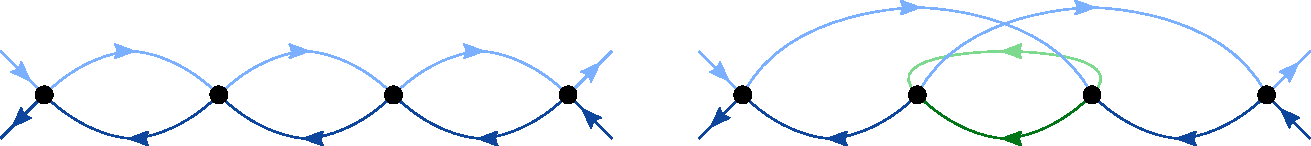
\includegraphics[scale=0.3]{diagrams/PT4_K1a}
\\
\phantom{.}\hspace{0.45cm} $\K1a$ ladder \hspace{1.5cm} $\K1a$ non-ladder
\\ \\
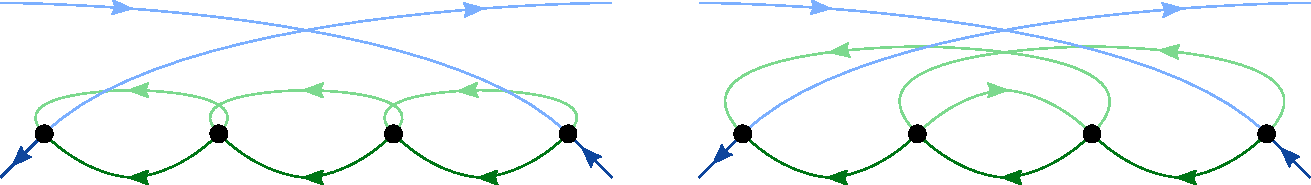
\includegraphics[scale=0.3]{diagrams/PT4_K1p}
\\
\phantom{.}\hspace{0.45cm} $\K1p$ ladder \hspace{1.5cm} $\K1p$ non-ladder
\\ \\
\phantom{.} \hspace{0.6cm}
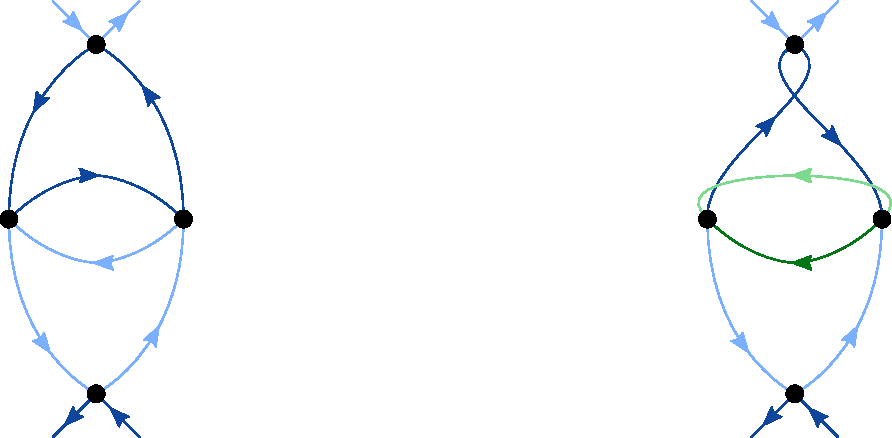
\includegraphics[scale=0.3]{diagrams/PT4_K1t}
\\
\phantom{.} \hspace{0.45cm} $(\Gamma_0,\K2t)$ \hspace{2.1cm} $(\Gamma_0,\K2a)$
\\
\phantom{.}\hspace{1.1cm} $\K1t$ non-ladder diagrams
\end{subfigure}
\begin{subfigure}[c]{0.4\textwidth}
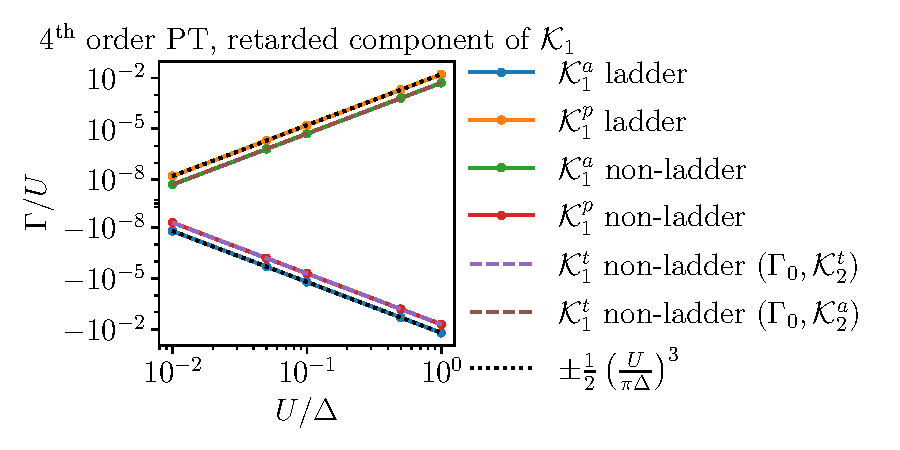
\includegraphics[scale=0.65]{plots/PT4_K1}
\end{subfigure}
\caption{$\Ktot1$ diagrams in $4^\text{th}$ order. In the $a$ and $p$ channel, diagrams can be split into ladder and non-ladder type diagrams. In the $t$ channel, the $\uparrow\downarrow$ component of the ladder diagram is zero. 
The ladder (non-ladder) diagrams in the $a$ and $p$ channel cancel (exact result is known for the ladder diagrams). The non-ladder diagrams in the $t$ channel cancel each other.}
\end{figure}

\subsubsection*{$\mathcal{K}_2$ diagrams}

$\Ktot{{2^{\prime}}}$ diagrams follow by mirroring the $\Ktot2$ diagrams along the vertical axis and give the same values, they are thus not depicted explicitly in $4^\text{th}$ order.

\begin{figure}[h!]
\begin{subfigure}[c]{0.4\textwidth}
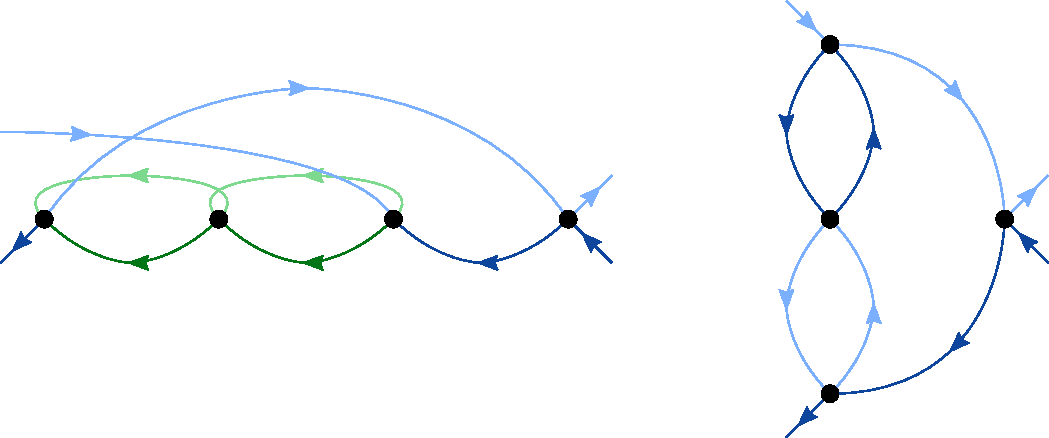
\includegraphics[scale=0.3]{diagrams/PT4_K2a_1}
\\
\phantom{.}\hspace{0.45cm} $\K2a \leftarrow \K1p, \Gamma_0$ \hspace{1cm} $\K2a \leftarrow \K1t, \Gamma_0$
\\ \\
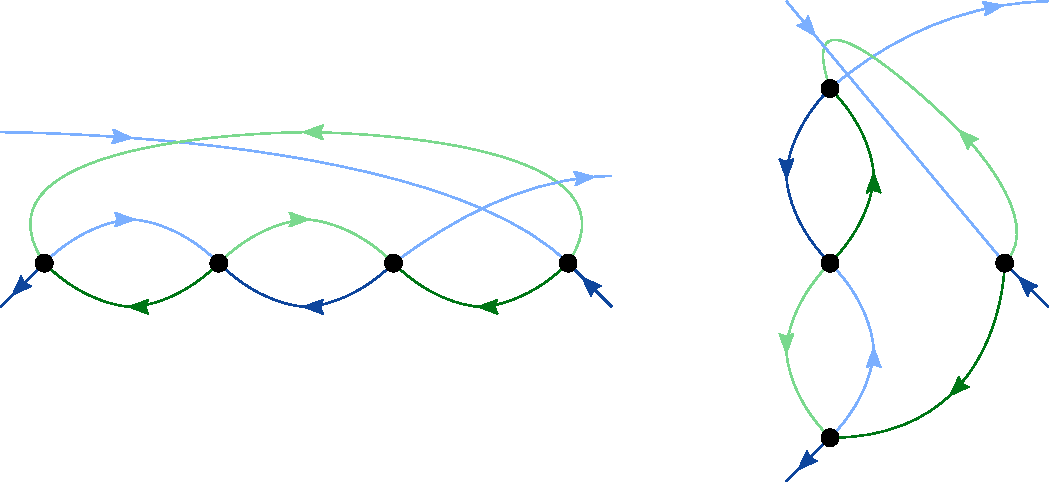
\includegraphics[scale=0.3]{diagrams/PT4_K2p_1}
\\
\phantom{.}\hspace{0.45cm} $\K2p \leftarrow \K1a, \Gamma_0$ \hspace{1cm} $\K2p \leftarrow \K1t, \Gamma_0$
\end{subfigure}
\begin{subfigure}[c]{0.4\textwidth}
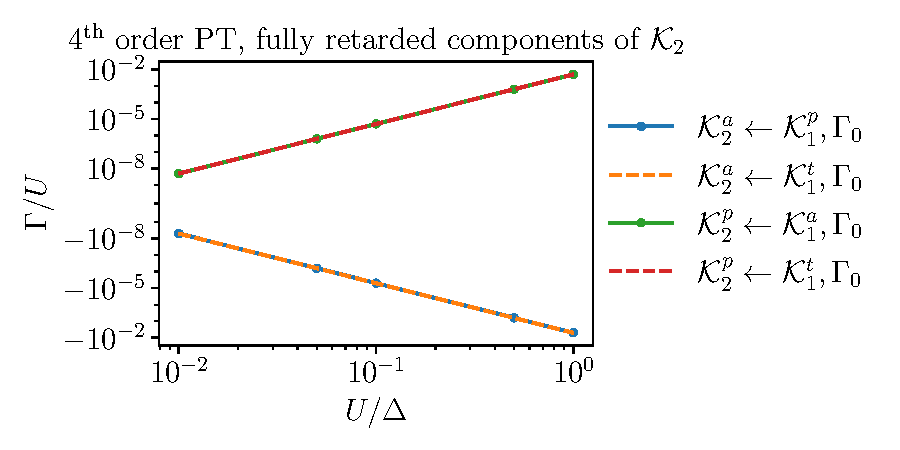
\includegraphics[scale=0.65]{plots/PT4_K2_1}
\end{subfigure}
\caption{$\Ktot2$ diagrams in $4^\text{th}$ order obtained by inserting a $3^\text{rd}$ order $\Ktot1$ diagram. Diagrams in the $a$ and $p$ channel cancel ($t$ diagrams are again zero due to the spin structure).}
\end{figure}

\newpage

\begin{figure}[h!]
\begin{subfigure}[c]{0.4\textwidth}
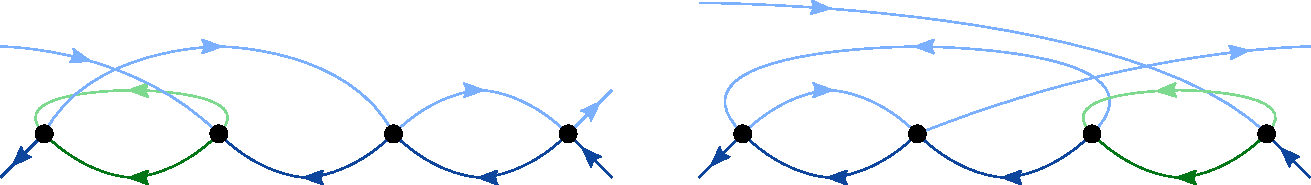
\includegraphics[scale=0.3]{diagrams/PT4_K2_2s_ap}
\\
\phantom{.}\hspace{0.45cm} $\K2a \leftarrow \K2a, \Gamma_0$ \hspace{1cm} $\K2p \leftarrow \K2p, \Gamma_0$
\\ \\
\phantom{.}\hspace{0.45cm}
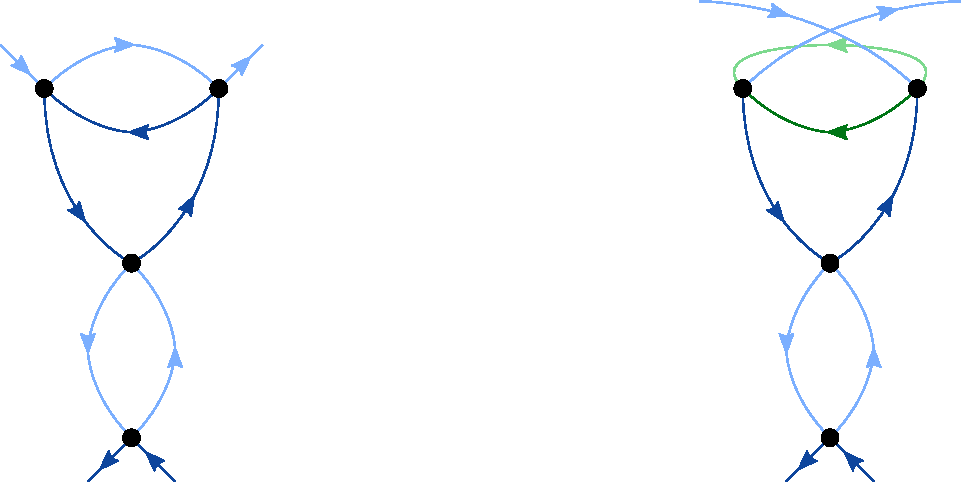
\includegraphics[scale=0.3]{diagrams/PT4_K2_2s_t}
\\
\phantom{.}$\K2t \leftarrow (\K1a, \Gamma_0), \Gamma_0$ \hspace{0.6cm} $\K2t \leftarrow (\K1p, \Gamma_0), \Gamma_0$
\end{subfigure}
\begin{subfigure}[c]{0.4\textwidth}
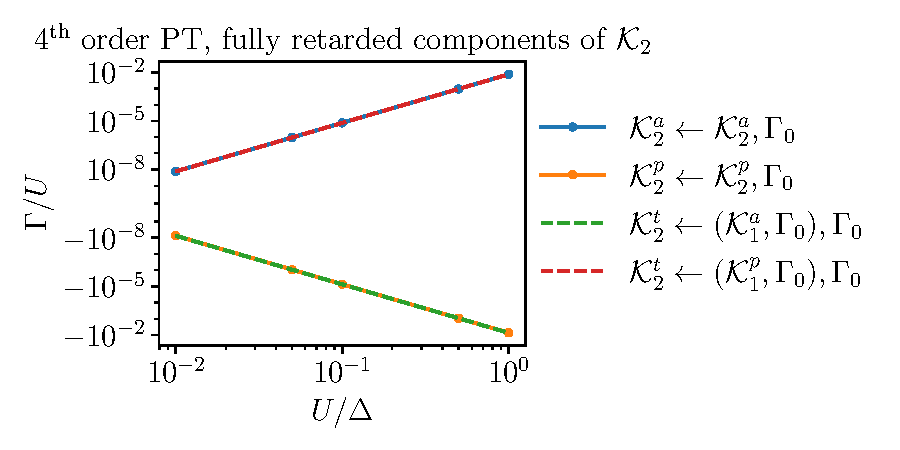
\includegraphics[scale=0.65]{plots/PT4_K2_2s}
\end{subfigure}
\caption{$\Ktot2$ diagrams in $4^\text{th}$ order obtained by inserting a $3^\text{rd}$ order $\K2r$ diagram in channel $r$. Diagrams in the $a$ and $p$ channel cancel, and the two $t$ diagrams cancel separately.}
\end{figure}


\begin{figure}[h!]
\begin{subfigure}[c]{0.4\textwidth}
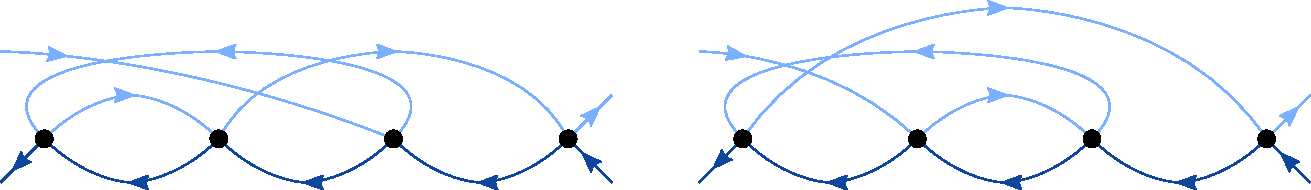
\includegraphics[scale=0.3]{diagrams/PT4_K2a_2d_p}
\\
\phantom{.}\hspace{0.45cm} $\K2a \leftarrow \K2p, \Gamma_0$ \hspace{1.1cm} $\K2a \leftarrow \Kb2p, \Gamma_0$
\\ \\
\phantom{.}\hspace{0.4cm}
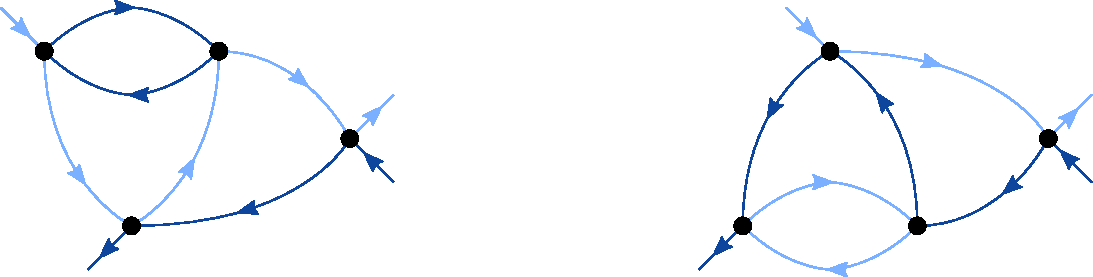
\includegraphics[scale=0.3]{diagrams/PT4_K2a_2d_t}
\\
\phantom{.}\hspace{0.45cm} $\K2a \leftarrow \K2t, \Gamma_0$ \hspace{1.1cm} $\K2a \leftarrow \Kb2t, \Gamma_0$
\\ \\
\\ \\
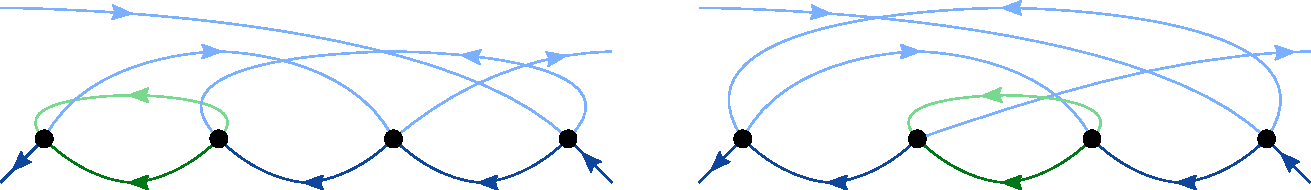
\includegraphics[scale=0.3]{diagrams/PT4_K2p_2d_a}
\\
\phantom{.}\hspace{0.45cm} $\K2p \leftarrow \K2a, \Gamma_0$ \hspace{1.1cm} $\K2p \leftarrow \Kb2a, \Gamma_0$
\\ \\
\phantom{.}\hspace{0.45cm}
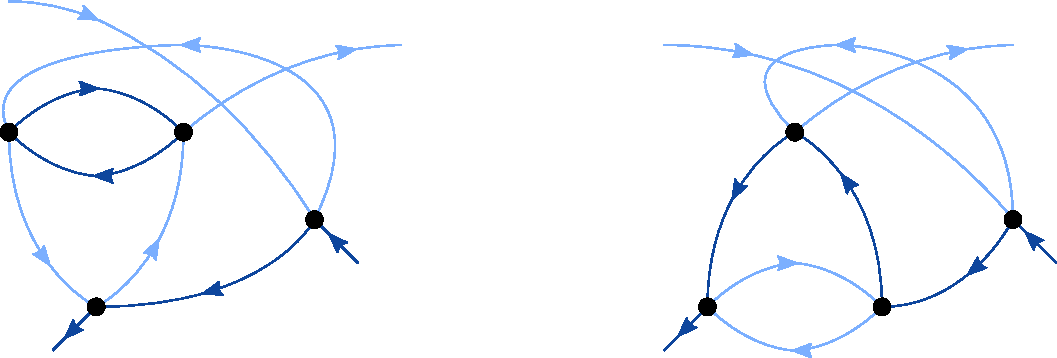
\includegraphics[scale=0.3]{diagrams/PT4_K2p_2d_t}
\\
\phantom{.}\hspace{0.45cm} $\K2p \leftarrow \K2t, \Gamma_0$ \hspace{1.1cm} $\K2p \leftarrow \Kb2t, \Gamma_0$
\end{subfigure}
\begin{subfigure}[c]{0.4\textwidth}
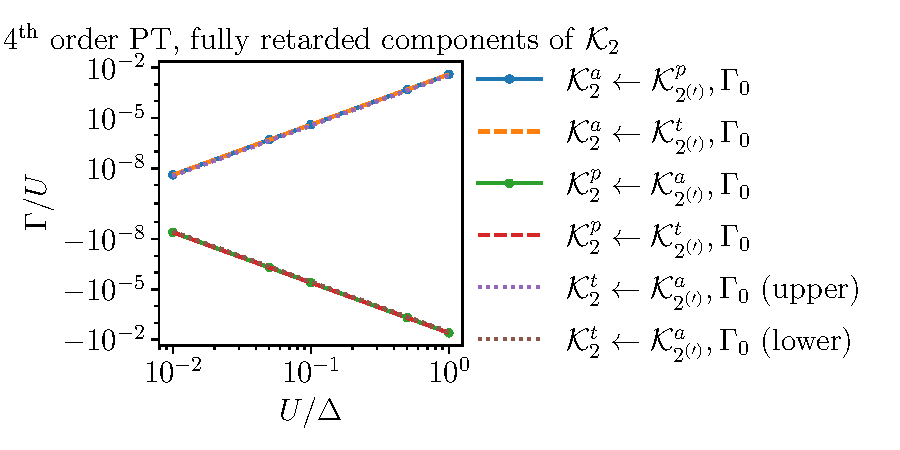
\includegraphics[scale=0.65]{plots/PT4_K2_2d}
\\
\phantom{.}\hspace{0.45cm}
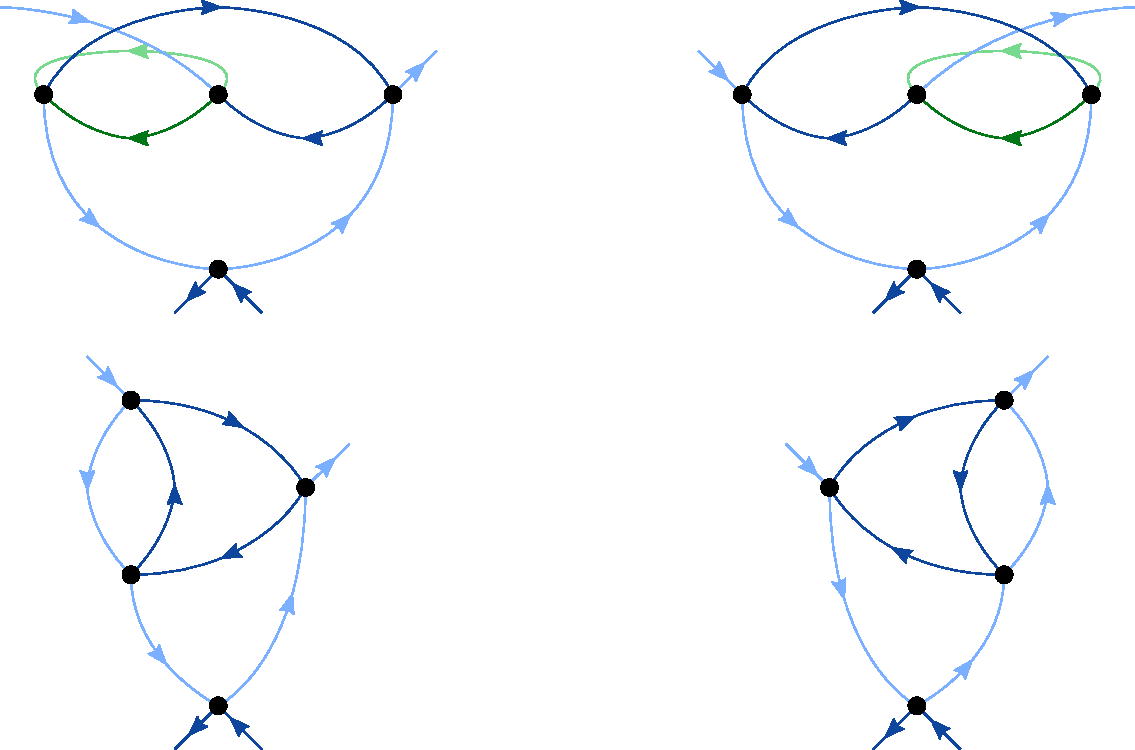
\includegraphics[scale=0.3]{diagrams/PT4_K2t_2d_a}
\\
\phantom{.}\hspace{0.6cm} $\K2t \leftarrow \K2a, \Gamma_0$ \hspace{1.4cm} $\K2t \leftarrow \Kb2a, \Gamma_0$
\end{subfigure}
\caption{$\Ktot2$ diagrams in $4^\text{th}$ order obtained by inserting a $3^\text{rd}$ order $\K{2}{{\bar{r}}}$ diagram in channel $r$. Diagrams in the $a$ and $p$ channel cancel. In the $t$ channel, the upper two diagrams (containing $\K1p$ in $2^\text{nd}$ order) and the lower two diagrams (containing $\K1t$ in $2^\text{nd}$ order) cancel. (Inserting $\K{{2^{(\prime)}}}{p}$ in $3^\text{rd}$ order in the $t$ channel gives zero due to the spin structure.)}
\end{figure}

\newpage

\subsubsection*{$\mathcal{K}_3$ diagrams}

\begin{figure}[h!]
\begin{subfigure}[c]{0.4\textwidth}
\phantom{.}\hspace{0.45cm}
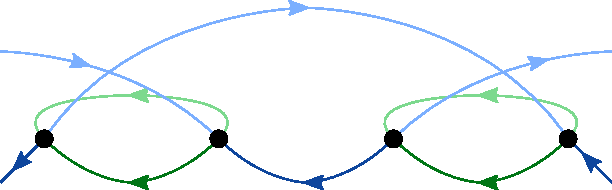
\includegraphics[scale=0.3]{diagrams/PT4_K3a}
\\
\phantom{.}\hspace{1.8cm} $\K3a$
\\ \\
\phantom{.}\hspace{0.45cm}
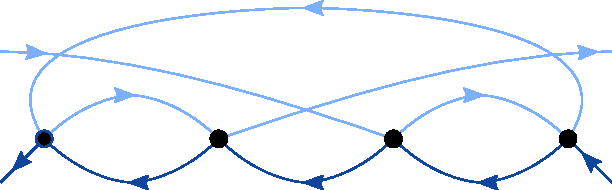
\includegraphics[scale=0.3]{diagrams/PT4_K3p}
\\
\phantom{.}\hspace{1.8cm} $\K3p$
\\ \\
\phantom{.}\hspace{0.45cm}
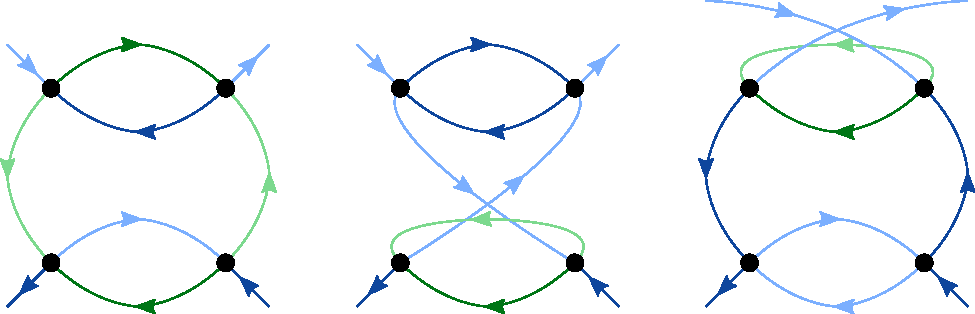
\includegraphics[scale=0.3]{diagrams/PT4_K3t}
\\
$\K3t$ \hspace{0.5cm} $a$-$a$ \hspace{1.05cm} $a$-$p$ \hspace{1.05cm} $p$-$a$
\end{subfigure}
\begin{subfigure}[c]{0.4\textwidth}
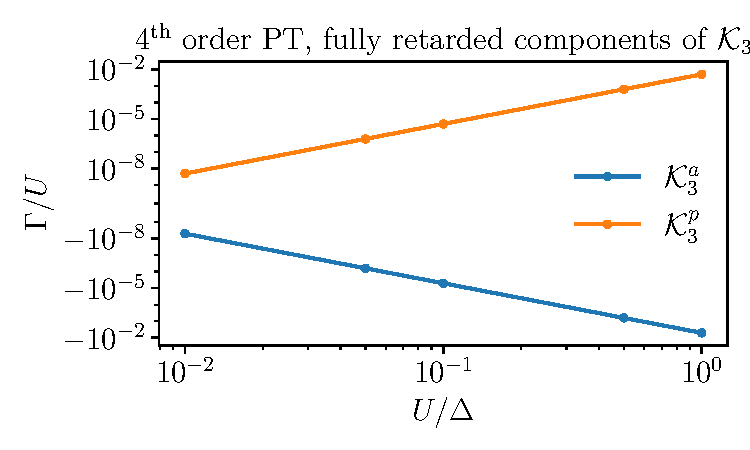
\includegraphics[scale=0.65]{plots/PT4_K3ap}
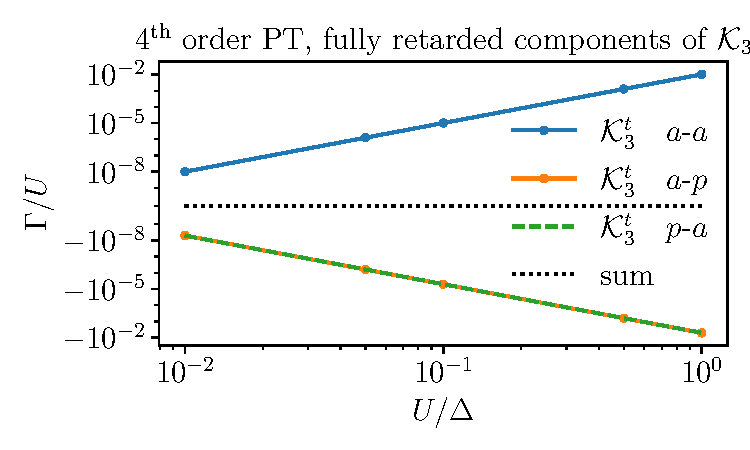
\includegraphics[scale=0.65]{plots/PT4_K3t}
\end{subfigure}
\caption{$\Ktot3$ diagrams in $4^\text{th}$ order. In the $t$ channel, one can insert $\K1a$ and $\K1p$ on both sides of the bubble. The $p$-$p$ insertion is zero due to the spin structure. Diagrams in the $a$ and $p$ channel cancel, and the three $t$ diagrams cancel separately. Notice that the $a$-$a$ diagram in $\K3t$ does \textit{not} come with a prefactor $1/2$ despite having an internal spin sum, since it does not contain any $p$ bubble. Therefore, it corresponds to two spin-resolved diagrams for the two possible spins of the green lines, in contrast to diagrams with a (green) $p$ bubble, where the prefactor $1/2$ effectively accounts for the spin sum.}
\end{figure}


\end{document}

